\documentclass[a4paper, 12pt]{article}

\usepackage{arxiv}

\usepackage[T2A]{fontenc}
\usepackage[utf8]{inputenc}
\usepackage[english, russian]{babel}
% \usepackage{cmap}
\usepackage{url}
\usepackage{booktabs}
\usepackage{nicefrac}
\usepackage{microtype}
\usepackage{lipsum}
\usepackage{graphicx}
\usepackage{epstopdf}
\usepackage{subfig}
\usepackage[square,sort,comma,numbers]{natbib}
\usepackage{doi}
\usepackage{multicol}
\usepackage{multirow}
\usepackage{tabularx}
\usepackage{float}

\usepackage{tikz}
\usetikzlibrary{matrix}

% Algorithms
\usepackage{algpseudocode}
\usepackage{algorithm}

%% Шрифты
\usepackage{euscript} % Шрифт Евклид
\usepackage{mathrsfs} % Красивый матшрифт
\usepackage{extsizes} % Возможность сделать 14-й шрифт
\usepackage{bm}

\usepackage{makecell} % diaghead in a table
\usepackage{amsmath,amsfonts,amssymb,amsthm,mathtools,dsfont}
\usepackage{icomma}
\usepackage[labelfont=bf]{caption}
\usepackage{subfig} % for subfigures
\usepackage{wrapfig}

\newcommand{\bz}{\mathbf{z}}
\newcommand{\bx}{\mathbf{x}}
\newcommand{\by}{\mathbf{y}}
\newcommand{\bv}{\mathbf{v}}
\newcommand{\bw}{\mathbf{w}}
\newcommand{\ba}{\mathbf{a}}
\newcommand{\bb}{\mathbf{b}}
\newcommand{\bp}{\mathbf{p}}
\newcommand{\bq}{\mathbf{q}}
\newcommand{\bt}{\mathbf{t}}
\newcommand{\bu}{\mathbf{u}}
\newcommand{\bs}{\mathbf{s}}
\newcommand{\bT}{\mathbf{T}}
\newcommand{\bX}{\mathbf{X}}
\newcommand{\bZ}{\mathbf{Z}}
\newcommand{\bS}{\mathbf{S}}
\newcommand{\bH}{\mathbf{H}}
\newcommand{\bW}{\mathbf{W}}
\newcommand{\bY}{\mathbf{Y}}
\newcommand{\bU}{\mathbf{U}}
\newcommand{\bQ}{\mathbf{Q}}
\newcommand{\bP}{\mathbf{P}}
\newcommand{\bA}{\mathbf{A}}
\newcommand{\bB}{\mathbf{B}}
\newcommand{\bC}{\mathbf{C}}
\newcommand{\bE}{\mathbf{E}}
\newcommand{\bF}{\mathbf{F}}
\newcommand{\bomega}{\boldsymbol{\omega}}
\newcommand{\btheta}{\boldsymbol{\theta}}
\newcommand{\bgamma}{\boldsymbol{\gamma}}
\newcommand{\bdelta}{\boldsymbol{\delta}}
\newcommand{\bPsi}{\boldsymbol{\Psi}}
\newcommand{\bpsi}{\boldsymbol{\psi}}
\newcommand{\bxi}{\boldsymbol{\xi}}
\newcommand{\bchi}{\boldsymbol{\chi}}
\newcommand{\bzeta}{\boldsymbol{\zeta}}
\newcommand{\blambda}{\boldsymbol{\lambda}}
\newcommand{\beps}{\boldsymbol{\varepsilon}}
\newcommand{\bZeta}{\boldsymbol{Z}}
% mathcal
\newcommand{\cX}{\mathcal{X}}
\newcommand{\cY}{\mathcal{Y}}
\newcommand{\cW}{\mathcal{W}}

\newcommand{\dH}{\mathds{H}}
\newcommand{\dR}{\mathds{R}}
% transpose
\newcommand{\T}{^{\mathsf{T}}}

% \renewcommand{\shorttitle}{\textit{arXiv} Шаблон}
\renewcommand{\epsilon}{\ensuremath{\varepsilon}}
\renewcommand{\phi}{\ensuremath{\varphi}}
\renewcommand{\kappa}{\ensuremath{\varkappa}}
\renewcommand{\le}{\ensuremath{\leqslant}}
\renewcommand{\leq}{\ensuremath{\leqslant}}
\renewcommand{\ge}{\ensuremath{\geqslant}}
\renewcommand{\geq}{\ensuremath{\geqslant}}
\renewcommand{\emptyset}{\varnothing}

\DeclareMathOperator*{\argmax}{arg\,max}  % in your preamble
\DeclareMathOperator*{\argmin}{arg\,min}  % in your preamble 

\usepackage{hyperref}
% \usepackage[usenames,dvipsnames,svgnames,table,rgb]{xcolor}

\hypersetup{
	unicode=true,
	colorlinks=true,
	linkcolor=black,        % внутренние ссылки
	citecolor=blue,         % на библиографию
	filecolor=magenta,      % на файлы
	urlcolor=blue           % на URL
}

\graphicspath{{./figures}}

\usepackage{enumitem} % Для модификаций перечневых окружений

\theoremstyle{definition} % "Определение"
\newtheorem{definition}{Опр.}[section]

\usepackage{etoolbox}

\makeatletter
\expandafter\patchcmd\csname\string\algorithmic\endcsname{\itemsep\z@}{\itemsep=1.5mm}{}{}
\makeatother

\newcommand{\myfigref}[2]{~\ref{#1}.\subref{#2}}% <---- a new macro for referring to a subfigure
\renewcommand{\abstractname}{Аннотация}

\title{Восстановление снимков фМРТ по просматриваемому видеоряду}

\author{
	%Дорин Даниил \\
	%\texttt{dorin.dd@phystech.edu} \\
	%\And
	Киселев Никита \\
	\texttt{kiselev.ns@phystech.edu} \\
	\And
	Грабовой Андрей \\
	\texttt{grabovoy.av@phystech.edu}
}
\date{\today}

\begin{document}
\maketitle

\begin{abstract}
	
	Исследуется проблема восстановления зависимости между показаниями датчиков фМРТ
	и восприятием внешнего мира человеком.
	Проводится анализ зависимости между последовательностью снимков фМРТ и видеорядом,
	просматриваемым человеком.
	На основе исследования зависимости предлагается метод аппроксимации показаний фМРТ по
	просматриваемому видеоряду.
	Для анализа предложенного метода проводится вычислительный эксперимент на 
	выборке, полученной при томографическом обследовании большого числа испытуемых.

\end{abstract}


\keywords{нейровизуализация \and фМРТ \and видеоряд \and зависимость между данными}

\section{Введение}

	Совокупность методов, визуализирующих структуру и функции человеческого мозга,
	называется \textit{нейровизуализацией}. Методы нейровизуализации, такие как ЭКГ, КТ, МРТ и фМРТ, 
	используются для изучения мозга, а также для обнаружения заболеваний и психических расстройств. 

	\textit{Функциональная магнитно-резонансная томография} или \textit{фМРТ} (англ.~\textit{fMRI}) 
	является разновидностью магнитно-резонансной томографии и основана на изменениях в токе крови, 
	вызванных нейронной активностью мозга \citep{Glover2011}. 
	Эти изменения происходят не моментально, а с некоторой задержкой.
	Она возникает из-за того, что сосудистая система достаточно долго реагирует 
	на потребность мозга в глюкозе \citep{Logothetis2003}. Изображения, получаемые с помощью фМРТ,
	показывают, какие участки мозга активированы при выполнении испытуемым определенных заданий.

	Настоящая работа посвящена восстановлению зависимости между снимками фМРТ и видеорядом.
	Используется предположение, что такая зависимость существует.
	Кроме того, предполагается, что между снимком и видеорядом есть постоянная задержка во времени
	\citep{Logothetis2003}.
	Проверяется зависимость снимка фМРТ от одного изображения и предыдущего снимка.
	Время задержки выступает в качестве гиперпараметра модели.
	На основе анализа зависимости предлагается метод аппроксимации показаний фМРТ по
	просматриваемому видеоряду.

	Метод фМРТ играет большую роль в нейровизуализации, однако имеет ряд важных ограничений.
	В работах \citep{menon1999spatial, logothetis2008we} рассматриваются 
	временное и пространственное разрешения фМРТ. Временное разрешение является существенным
	недостатком данного метода. Другой недостаток фМРТ~--- неизбежно возникающие шумы, 
	связанные с движением объекта в сканере, сердцебиением и дыханием человека, тепловыми
	флуктуациями самого прибора и т.\,д. В работе \citep{1804.10167} предлагаются методы 
	подавления вышеперечисленных шумов на основе графов и демонстрируется их эффективность в задаче
	выявления эпилепсии и депрессии.

	Обобщением уже естественных для обработки изображений 2D сверток в CNN являются 3D
	свертки \citep{Tran_2015_ICCV}.
	Они агрегируют информацию как по времени, так и по пространству.
	Однако это приводит к сильному увеличению количества используемых параметров.
	В~настоящей работе используется наиболее современная архитектура~--- Transformer.
	Впервые она была предложена в статье \citep{https://doi.org/10.48550/arxiv.1706.03762}.
	Не так давно появилась адаптация архитектуры Transformer для работы с видео
	\citep{https://doi.org/10.48550/arxiv.2201.04288}. Данная архитектура состоит из кодировщика
	и декодировщика, каждый из которых в свою очередь состоит из отдельных слоев. Использование 
	механизма Attention \citep{https://doi.org/10.48550/arxiv.1706.03762} 
	позволяет значительно повысить качество работы модели.

	Данные, на которых проводятся проверка гипотезы зависимости и демонстрация работы построенного 
	метода, представлены в работе \citep{Berezutskaya2022}. Этот набор данных был получен при
	обследовании группы из 63 испытуемых. Тридцать из них проходили обследование фМРТ.
	Им предлагалось выполнить одно и то же задание~--- просмотреть короткий аудиовизуальный фильм. 
	Для него в рассматриваемой работе были сгенерированы аннотации, содержащие в том числе информацию о времени появления и исчезновения
	отдельных слов, объектов и персонажей. Методы аудио- и видеоаннотирования подробно излагаются в
	\citep{boersma2018praat} и \citep{Berezutskaya2020}. 

\section{Постановка задачи}

	Задана частота кадров $\nu \in \mathbb{R}$ и продолжительность $t \in \mathbb{R}$ видеоряда. 
	Задан видеоряд
	\begin{equation}
		\label{eq1}
		\bP = [\bp_1, \ldots, \bp_{\nu t}], \quad\
		\bp_{\ell} \in \mathbb{R}^{W \times H \times C},
	\end{equation}
	с шириной, высотой и числом каналов изображения $W, H$ и 
	$C$ соответственно.

	Обозначим частоту снимков фМРТ $\mu \in \mathbb{R}$. Задана последовательность снимков 
	\begin{equation}
		\label{eq2}
		\bS = [\bs_1, \ldots, \bs_{\mu t}], \quad\
		\bs_{\ell} \in \mathbb{R}^{X \times Y \times Z},
	\end{equation}
	где $X, Y$ и $Z$~--- размерности воксельного изображения. 

	Задача состоит в построении отображения, которое бы учитывало задержку $\Delta t$ между
	снимком фМРТ и видеорядом, а также предыдущие томографические показания. Формально, необходимо
	найти такое отображение $\mathbf{g}$, что
	\begin{equation}
		\label{eq3}
		\mathbf{g}(\bp_1, \ldots, \bp_{k_{\ell} - \nu \Delta t}; \bs_1, \ldots, \bs_{\ell-1}) = \bs_{\ell},
		\ \ell = 1, \ldots, \mu t,
	\end{equation}
	где для $\ell$-го снимка фМРТ номер соответствующего изображения $k_{\ell}$ определяется по формуле
	\begin{equation}
		\label{eq4}
		k_{\ell} = \dfrac{\ell \cdot \nu}{\mu}.
	\end{equation}

\section{Предлагаемый метод восстановления снимков фМРТ}

	Обозначим снимок фМРТ как $\bs_{\ell} = [v^{\ell}_{ijk}] \in \mathbb{R}^{X \times Y \times Z}$,
	где $v^{\ell}_{ijk} \in \mathbb{R}_+$~--- значение соответствующего вокселя.
	Предположим, что каждый снимок зависит только от одного изображения и предыдущего снимка.
	Тогда соответствующее отображение можно записать в виде
	\begin{equation}
		\label{eq5}
		\mathbf{g}(\bp_{k_{\ell} - \nu \Delta t}; \bs_{\ell-1}) = \bs_{\ell} - \bs_{\ell-1} = \bdelta_{\ell}, \ \ell = 2, \ldots, \mu t.
	\end{equation}
	где $\bdelta_{\ell} = [v^{\ell}_{ijk} - v^{\ell-1}_{ijk}] = [\delta^{\ell}_{ijk}] \in \mathbb{R}^{X \times Y \times Z}$~--- разность между двумя последовательными снимками.

	Для каждого изображения из видеоряда имеем вектор признакового описания размерности $d$:
	\[ \bx_{\ell} = [x^{\ell}_1, \ldots, x^{\ell}_{d}]\T \in \mathbb{R}^{d}, \ {\ell} = 1, \ldots, \nu t. \]
	Используется архитектура нейронной сети ResNet152 без последнего линейного слоя.

	Учитывая \eqref{eq4}, суммарное число пар (изображение, снимок) 
	равно $N = \mu (t - \Delta t)$. Таким образом, для каждого вокселя задана выборка
	\[ \mathfrak{D}_{ijk} = \{(\bx_{\ell}, \delta^{\ell}_{ijk}) \ | \ {\ell} = 2, \ldots, N \}. \]

	Поставлена задача восстановления регрессии
	\begin{equation}
		\label{eq6}
		y_{ijk}: \mathbb{R}^{d} \to \mathbb{R}.
	\end{equation}
		
	Используется линейная модель с вектором параметров 
	\[ \bw_{ijk} = [w^{ijk}_1, \ldots, w^{ijk}_{d}]\T \in \mathbb{R}^{d}: \]
	\begin{equation}
		\label{eq7}
		f_{ijk}(\bx, \bw_{ijk}) = \langle \bx, \bw_{ijk} \rangle.
	\end{equation}

	Для модели $f_{ijk}$ с соответствующим ей вектором параметров $\bw_{ijk} \in \mathbb{R}^{d}$
	определим квадратичную функцию потерь с $L_2$ регуляризацией:
	\begin{equation}
		\label{eq8}
		\mathcal{L}_{ijk}(\bw_{ijk}, \Delta t) = \sum\limits_{\ell = 2}^{N} \big(f_{ijk}(\bx_{\ell}, \bw_{ijk}) - \delta^{\ell}_{ijk}\big)^2 + \alpha \| \bw_{ijk} \|_2^2,
	\end{equation}
	где $\alpha \in \mathbb{R}$~--- коэффициент регуляризации.

	Требуется найти параметры, доставляющие минимум функционалу потерь $\mathcal{L}_{ijk}(\bw_{ijk}, \Delta t)$
	при заданном гиперпараметре $\Delta t$:
	\begin{equation}
		\label{eq9}
		\hat{\bw}_{ijk} = \argmin_{\bw_{ijk}} \mathcal{L}_{ijk}(\bw_{ijk}, \Delta t).
	\end{equation}

	Минимум функции потерь находится методом наименьших квадратов. Определим матрицу объектов-признаков
	\begin{equation}
		\label{eq10}
		\bX = [\bx_2\T, \ldots, \bx_N\T]\T = [x^i_j] \in \mathbb{R}^{(N-1) \times d}
	\end{equation}
	и вектор, компонентами которого являются разности значений одного и того же вокселя в разных снимках,
	\begin{equation}
		\label{eq11}
		\mathbf{\Delta v}_{ijk} = [\delta^2_{ijk}, \ldots, \delta^N_{ijk}]\T \in \mathbb{R}^{N-1}.
	\end{equation}

	Решение можно записать в виде
	\begin{equation}
		\label{eq12}
		\hat{\bw}_{ijk} = (\bX\T \bX + \alpha \mathbf{I})^{-1} \bX\T \mathbf{\Delta v}_{ijk}.
	\end{equation}

	Получим формулу для восстановленных снимков фМРТ. Введем матрицу весов
	\begin{equation}
		\label{eq13}
		\hat{\bW} = [\hat{\bw}_1\T, \ldots, \hat{\bw}_{XYZ}\T]\T = [\hat{w}^i_j] \in \mathbb{R}^{XYZ \times d}.
	\end{equation}

	Введем для тензоров $\bs_{\ell}, \bdelta_{\ell} \in \mathbb{R}^{X \times Y \times Z}$ векторы
	\[ \bs_{\ell}^{R} = [ v^{\ell}_1, \ldots, v^{\ell}_{XYZ} ]\T,\
	\bdelta_{\ell}^{R} = [ \delta^{\ell}_1, \ldots, \delta^{\ell}_{XYZ} ]\T \in \mathbb{R}^{XYZ}. \]

	Тогда вектор восстановленного снимка находится по формуле
	\begin{equation}
		\label{eq14}
		\hat{\bs}_{\ell}^{R} = \bs_{\ell-1}^{R} + \hat{\bdelta}_{\ell}^{R} = \bs_{\ell-1}^{R} + \hat{\mathbf{W}} \mathbf{x}_{\ell}.
	\end{equation}

\section{Вычислительный эксперимент}

	Для анализа работоспособности предложенного метода, а также проверки гипотез 
	проведен вычислительный эксперимент.

	В качестве данных использовалась выборка, представленная в работе \citep{Berezutskaya2022}.
	Набор данных содержит результаты обследования 63 испытуемых.
	Для тридцати из них известны показания фМРТ.
	Среди них 16 мужчин и 14 женщин в возрасте от 7 до 47 лет.
	Средний возраст испытуемого~--- 22 года.

	Размерности изображений и снимков, а также другие характеристики выборки представлены в 
	Таблице~\ref{table:sample}.

	\begin{table}
		\centering
		\caption{Описание выборки}
		\begin{tabular}{|c|c|c|}
			\hline
			Название & Обозначение & Значение \\
			\hline \hline
			Продолжительность обследования & $t$ & 390 с \\ \hline
			Частота кадров видео & $\nu$ & 25 $\text{с}^{-1}$ \\ \hline
			Частота снимков фМРТ & $\mu$ & 1,64 $\text{с}^{-1}$ \\ \hline
			Размерности изображения & $W, H, C$ & 640, 480, 3 \\ \hline
			Размерности снимка & $X, Y, Z$ & 40, 64, 64 \\ \hline
		\end{tabular}
		\label{table:sample}
	\end{table}

	Произведено разделение выборки на тренировочную и тестовую в соотношении 70\% и 30\% соответственно.
	Критерием качества восстановления снимка фМРТ служит MSE~--- сумма квадратов отклонений 
	между истинным и восстановленным снимками, усредненная по всем вокселям каждого снимка
	из тестовой выборки.

	Для сокращения времени работы алгоритма производится предварительное сжатие снимка фМРТ
	с помощью сверточного слоя MaxPool3D. Рассматриваются коэффициенты сжатия 1, 2, 4 и 8.
	Значения вокселей нормализуются на $[0; 1]$ процедурой MinMaxScale.

	Проанализирована зависимость качества восстановления снимков фМРТ от гиперпараметра $\Delta t$.
	Использовалось предварительное 8-кратное сжатие снимка.
	Зависимость метрики MSE от гиперпараметра $\Delta t$ представлена на Рис.~\ref{fig:mse-dt}.
	Для построения графика производилось усреднение по испытуемым.
	Обозначены границы среднеквадратичного отклонения. 
	Наблюдается характерный минимум при $\Delta t \approx 10 \text{ с}$.
	
	\begin{figure}[h!]
		\centering
		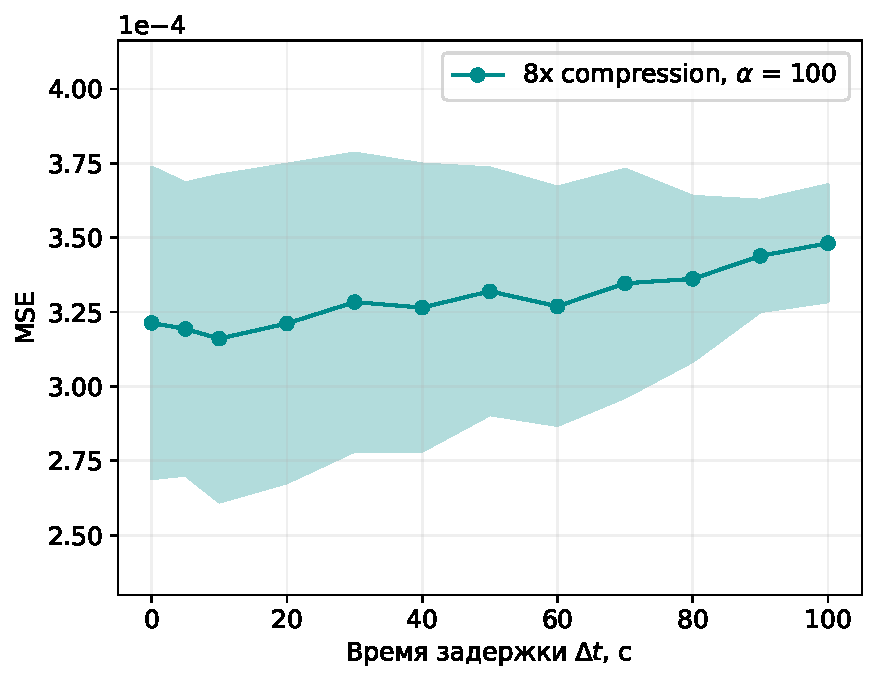
\includegraphics[width=0.65\textwidth]{subs_delta_MSE_dt.pdf}
		\caption{Зависимость метрики MSE от гиперпараметра $\Delta t$ на снимках из тестовой выборки}
		\label{fig:mse-dt}
	\end{figure}
	
	На Рис.~\ref*{fig:4} представлены срезы истинного и восстановленного снимков из 
	тестовой выборки. На Рис.\myfigref{fig:4}{fig:4c} можно наблюдать разность между ними.
	Был выбран 4-ый испытуемый, $\Delta t = 5 \text{ с}$, коэффициент сжатия 1, коэффициент регуляризации
	$\alpha = 1000$. Рассмотрен 20-ый срез по первому измерению 100-го снимка в последовательности.
	Значения вокселей лежат в отрезке $[0; 1]$, поэтому ошибка порядка $10^{-3} \div 10^{-2}$
	свидетельствует о достаточно точном предсказании.

	\begin{figure}[h!]
		\centering
		\subfloat[Истинный]{\label{fig:4a}{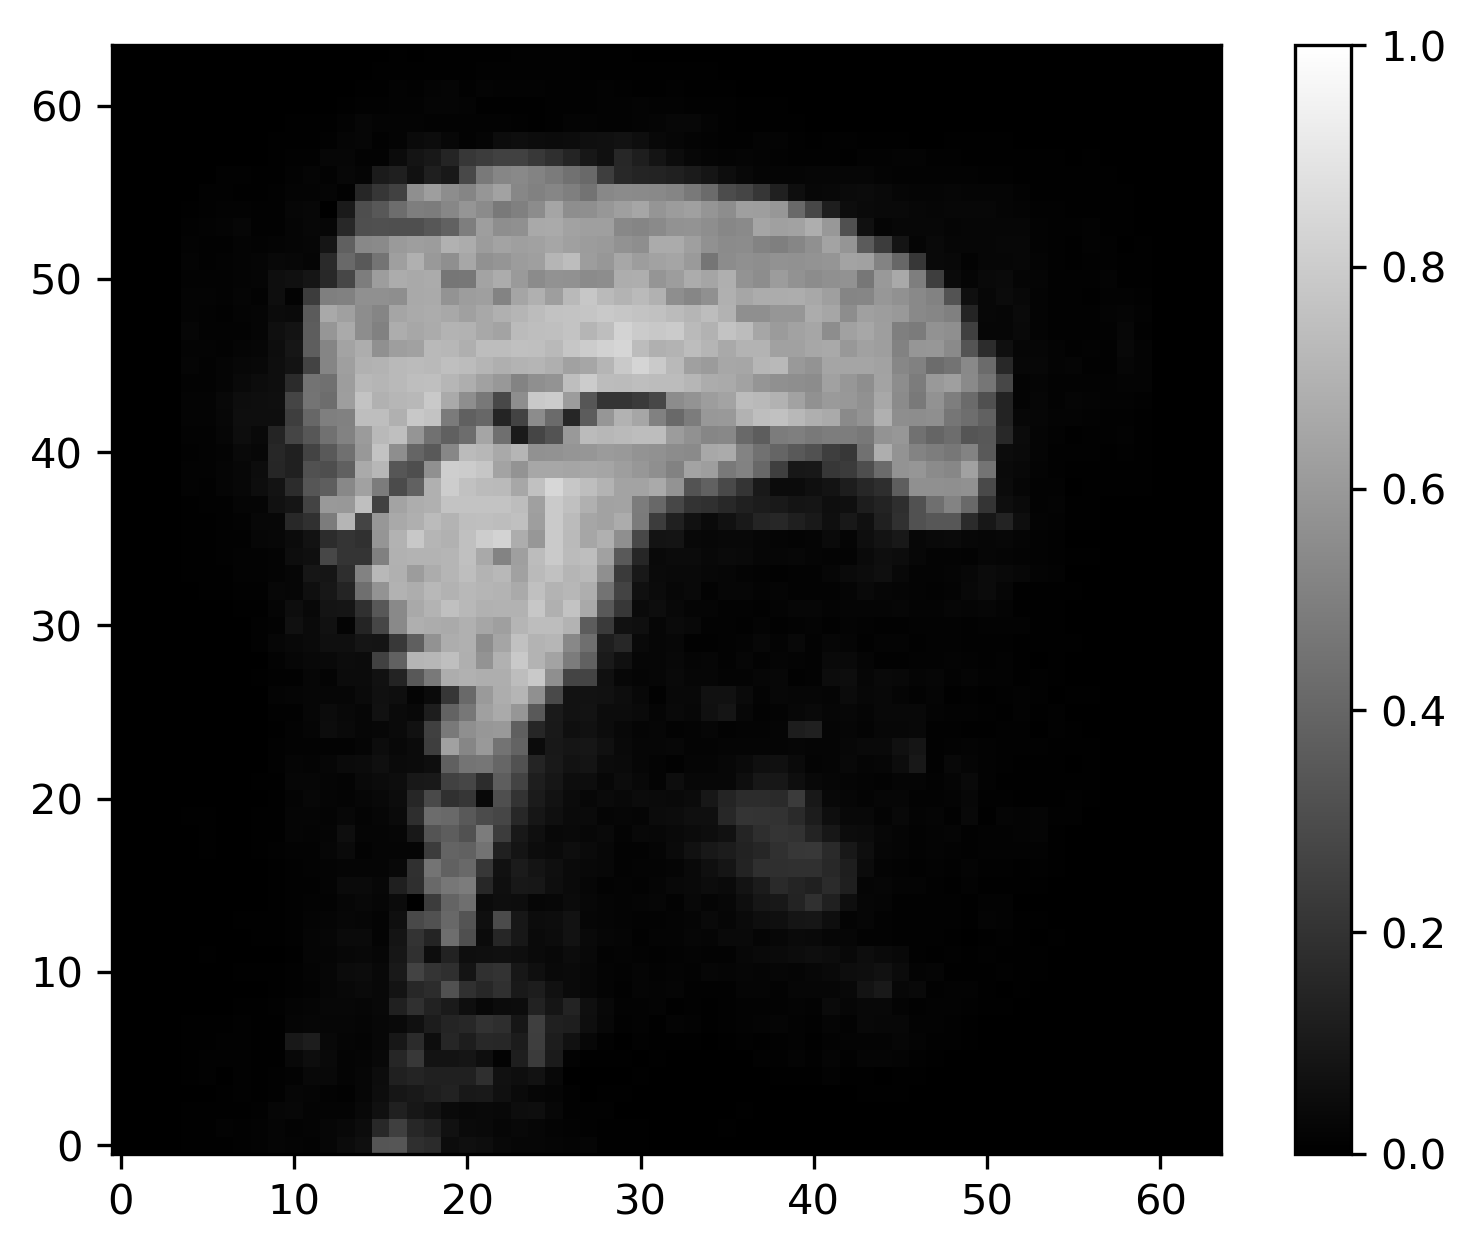
\includegraphics[width=0.33\textwidth]{sub-04-5-1-1000/sub-04-5-1-1000-100-20-_-_-test.png}}}
		\hfill
		\subfloat[Восстановленный]{\label{fig:4b}{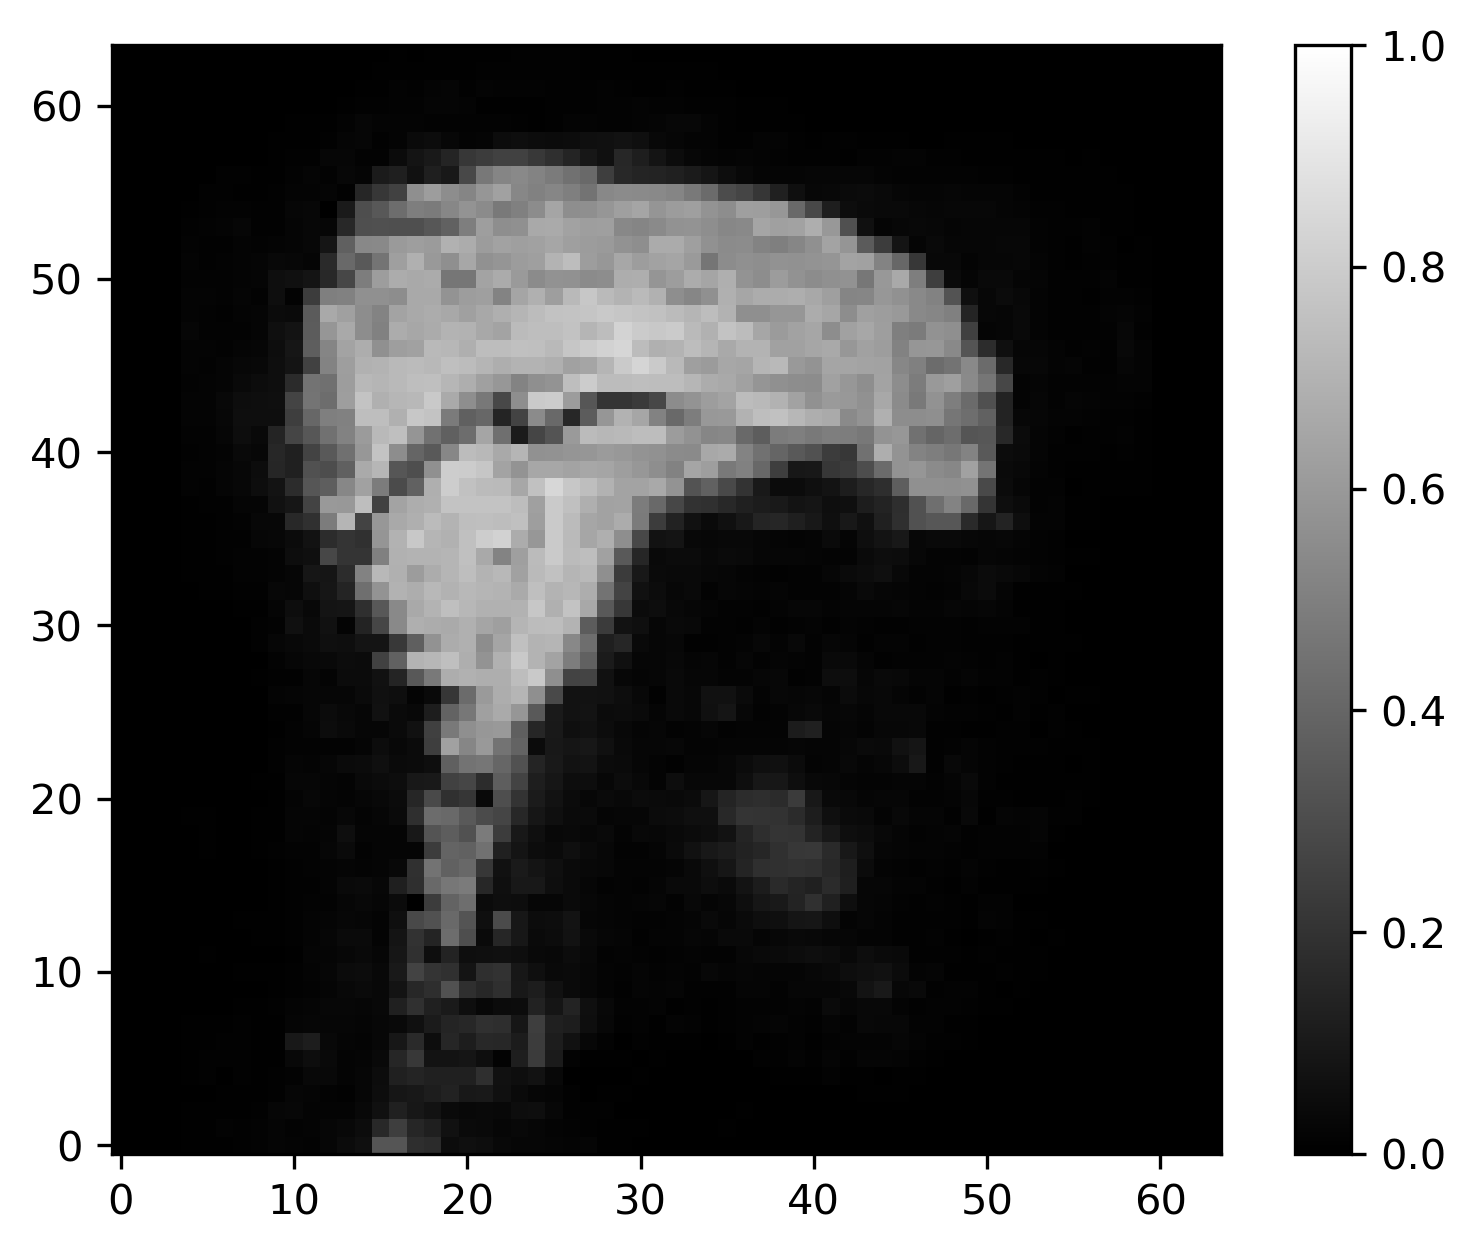
\includegraphics[width=0.33\textwidth]{sub-04-5-1-1000/sub-04-5-1-1000-100-20-_-_-predicted.png}}}
		\hfill
		\subfloat[Разность]{\label{fig:4c}{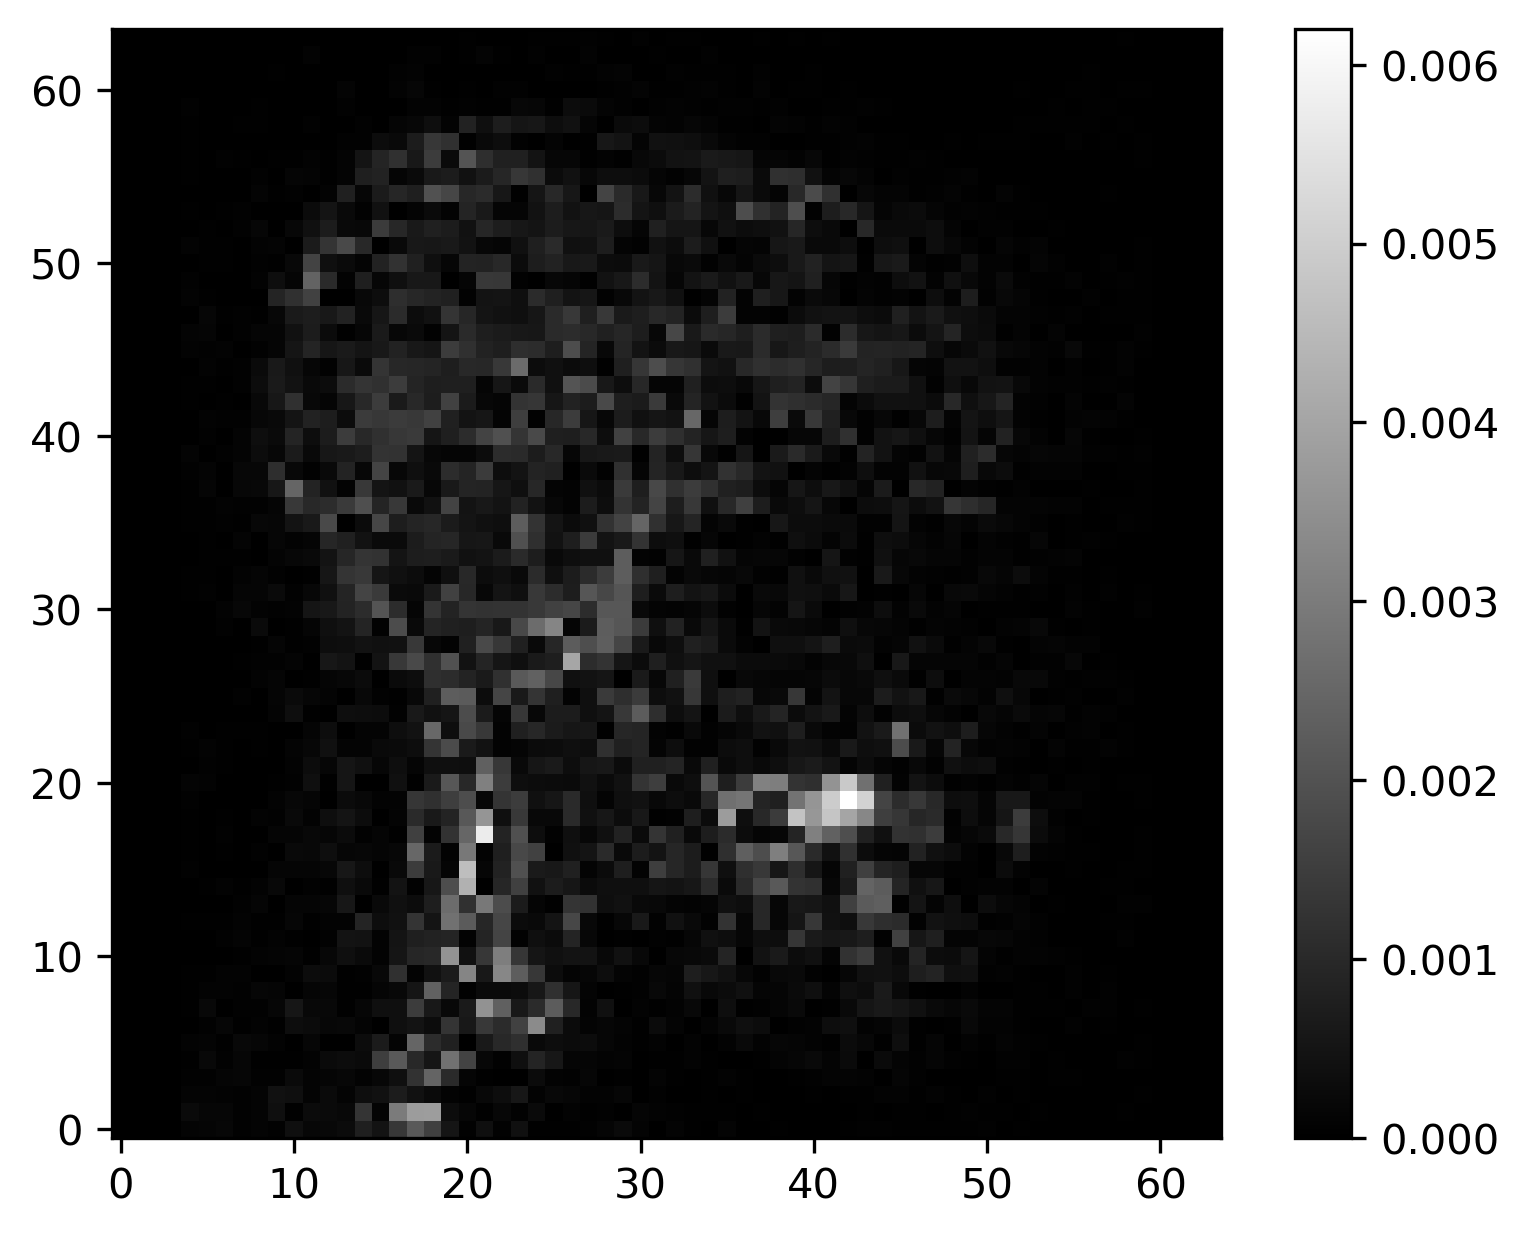
\includegraphics[width=0.33\textwidth]{sub-04-5-1-1000/sub-04-5-1-1000-100-20-_-_-difference.png}}}
		\caption{Срез снимка фМРТ из тестовой выборки}
		\label{fig:4}
	\end{figure}

	Проведен анализ зависимости MSE от коэффициента регуляризации $\alpha$.
	Рассматривались коэффициенты сжатия 1, 2, 4 и 8. 
	Соответствующие графики приведены на Рис.~\ref{fig:5}.
	Для построения графика производилось усреднение по испытуемым.
	Обозначены границы среднеквадратичного отклонения.
	Из графиков видно, что оптимальное значение коэффициента $\alpha \approx 100$.

	\begin{figure}[h!]
		\centering
		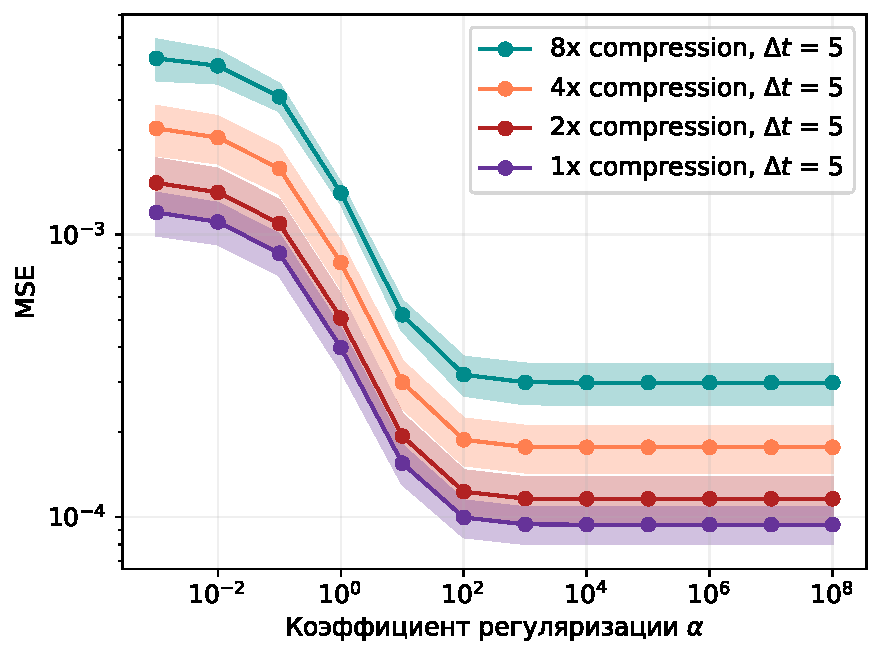
\includegraphics[width=0.65\textwidth]{subs_MSE_alpha.pdf}
		\caption{Зависимость метрики MSE от коэффициента регуляризации $\alpha$ на снимках из тестовой выборки}
		\label{fig:5}
	\end{figure}

	Построен график распределения значений компонент вектора весов модели.
	Для построения производилось усреднение по всем вокселям для 4-го испытуемого.
	Результат представлен на Рис.~\ref{fig:6}.
	Веса модели не лежат в окрестности какого-то конкретного значения, а распределены нормально.
	Это может говорить о том, что построенная модель, вероятно, имеет определенную
	статистическую значимость.

	\begin{figure}[h!]
		\centering
		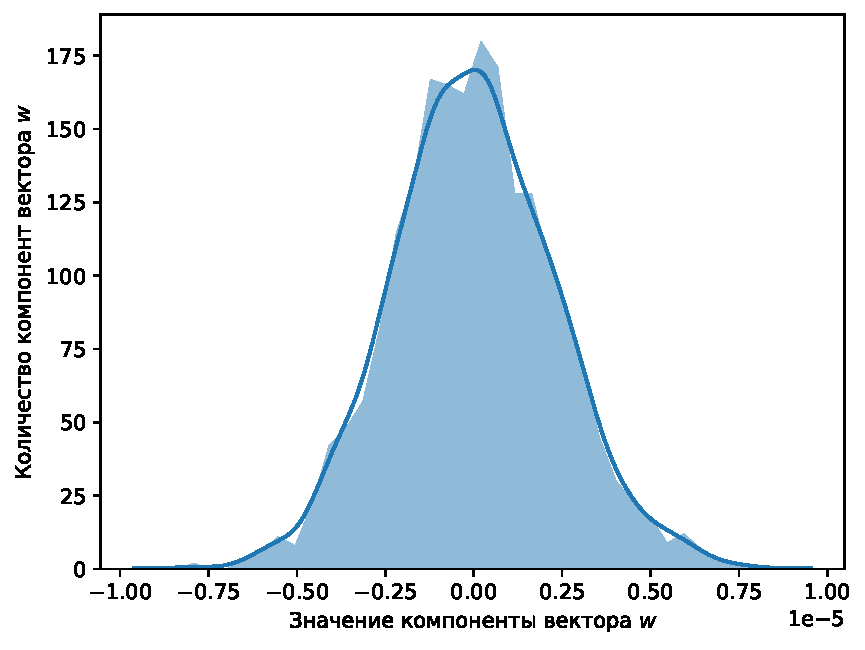
\includegraphics[width=0.65\textwidth]{mean_weight_distribution.pdf}
		\caption{Распределение значений компонент вектора весов}
		\label{fig:6}
	\end{figure}

	Проведена проверка гипотезы инвариантности весов модели относительно человека:
	можно ли восстановление снимка фМРТ одного испытуемого, используя
	матрицу весов другого. Использовалась метрика MSE на тестовой выборке.
	Результаты представлены в Таблице~\ref{table:inv}.
	Рассмотрены 4-ый и 7-ый испытуемые. Матрица весов 4-го использовалась для восстановления
	снимков 7-го.
	Значения MSE практически совпадает. Это свидетельствует о справедливости рассматриваемой
	гипотезы.

	\begin{table}[h!]
		\centering
		\caption{Проверка гипотезы инвариантности весов модели относительно человека}
		\begin{tabular}{|c|c|c|}
			\hline
			Матрица весов	&	Истинная	&	Подмешанная \\ \hline \hline
			MSE		& 	$1.02 \cdot 10^{-4}$	 &		$1.05 \cdot 10^{-4}$ \\ \hline
		\end{tabular}
		\label{table:inv}
	\end{table}

	Рассмотрено качество работы метода на случайном шуме. В качестве матрицы $\bX$ из \eqref{eq10}
	взята матрица случайных чисел из равномерного распределения на $[0; 1)$. 
	Произведено сравнение с результатами на настоящей матрице объектов-признаков. 
	К первому снимку 35-го испытуемого последовательно прибавляются все восстановленные 
	изменения значений вокселей. 
	В результате имеем последний снимок последовательности. На Рис.~\ref*{fig:7}
	представлены срезы последнего истинного и восстановленного снимков из тестовой выборки. 
	На Рис.\myfigref{fig:7}{fig:7c} можно наблюдать разность между ними.
	Результаты на случайном шуме продемонстрированы на Рис.~\ref*{fig:8}.
	Можно видеть, что разность между истинным и восстановленным снимками при работе со случайным шумом
	значительно выше. Численные результаты приведены в Таблице~\ref{table:2}.

	\begin{figure}[h!]
		\centering
		\subfloat[Истинный]{\label{fig:7a}{\includegraphics[width=0.33\textwidth]{sub-35-5-1-1000/original/sub-35-5-1-1000--1-20-_-_-recovered-test.png}}}
		\hfill
		\subfloat[Восстановленный]{\label{fig:7b}{\includegraphics[width=0.33\textwidth]{sub-35-5-1-1000/original/sub-35-5-1-1000--1-20-_-_-recovered-predicted.png}}}
		\hfill
		\subfloat[Разность]{\label{fig:7c}{\includegraphics[width=0.33\textwidth]{sub-35-5-1-1000/original/sub-35-5-1-1000--1-20-_-_-recovered-difference.png}}}
		\caption{Срез снимка фМРТ из тестовой выборки}
		\label{fig:7}
	\end{figure}

	\begin{figure}[h!]
		\centering
		\subfloat[Истинный]{\label{fig:8a}{\includegraphics[width=0.33\textwidth]{sub-35-5-1-1000/noised/sub-35-5-1-1000--1-20-_-_-recovered-test.png}}}
		\hfill
		\subfloat[Восстановленный]{\label{fig:8b}{\includegraphics[width=0.33\textwidth]{sub-35-5-1-1000/noised/sub-35-5-1-1000--1-20-_-_-recovered-predicted.png}}}
		\hfill
		\subfloat[Разность]{\label{fig:8c}{\includegraphics[width=0.33\textwidth]{sub-35-5-1-1000/noised/sub-35-5-1-1000--1-20-_-_-recovered-difference.png}}}
		\caption{Срез снимка фМРТ из тестовой выборки (на случайном шуме)}
		\label{fig:8}
	\end{figure}

	\begin{table}[h!]
		\centering
		\caption{Качество работы метода на случайном шуме}
		\begin{tabular}{|c|c|c|}
			\hline
			Выборка	&	Истинная	&	Случайный шум \\ \hline \hline
			MSE		& 	$2 \cdot 10^{-3}$	 &		$10^{-1}$ \\ \hline
		\end{tabular}
		\label{table:2}
	\end{table}

\newpage

\section{Заключение}

	Построен метод аппроксимации последовательности снимков фМРТ по видеоряду,
	просматриваемому человеком.
	Справедлива гипотеза о линейной зависимости между данными.
	Подтверждена гипотеза о взаимосвязи снимков в последовательности.
	Проверена гипотеза инвариантности весов модели относительно человека.

\newpage

\bibliographystyle{plain}
\bibliography{Kiselev2023fMRI.bib}

\end{document}